\chapter{The Longest Chain Protocol}
\label{sec:background}
% In this section, we review Nakamoto's longest chain protocol~\cite{bitcoin} and discuss the fundamental limitations in scaling its latency and throughput. These limitations motivate \prism's design, as we discuss in the next section. 

% %as a natural design to remove these limitations. 
% %%We will explain the design of \prism incrementally, first addressing throughput and then latency.



% \subsection{The longest chain protocol}

The most basic blockchain consensus protocol is Nakamoto's longest chain protocol, used in many systems including \bitcoin and \ethereum.  The basic object is a {\em block}, consisting of {\em transactions} and a reference link to another block. 
%A transaction is a payment signed by a sender's public key, and addressed to a recipient's public key. 
As transactions arrive into the system, a set of nodes, called {\em miners}, construct blocks and broadcast them to other nodes. The goal of the protocol is for all nodes to reach consensus on an ordered log of blocks (and the transactions therein), referred to as the {\em ledger}.

Starting with the {\em genesis} block as the root, each new block mined by a miner is added to create an evolving {\em blocktree}. In the longest chain protocol, honest miners append each block to the leaf block of the longest chain\footnote{In case of variable proof of work, honest miners mine on the "heaviest chain".} in the current blocktree, and the transactions in that block are added to the transaction ledger maintained by the blocks in the longest chain. 
A miner earns the right to append a block after solving a cryptographic puzzle, which requires finding a solution to a hash inequality.
 %the leaf block \ma{and the contents of the block being mined?}.  
 The miner includes the solution in the block as a {\em proof of work} (PoW), which other nodes can verify.  The time to solve the puzzle is random and exponentially distributed, with a mining rate $f$ that can be tuned by adjusting the difficulty of the puzzle. How fast an individual miner can solve the puzzle and mine the block is proportional to its hashing power, i.e. how fast it can compute hashes. 
 
 A block is confirmed to be in the ledger when it is $k$-deep in the ledger, i.e. the block is on the longest chain and a chain of $k-1$ blocks have been appended to it. It is proven that as long as the adversary has less than $50\%$ hashing power, the ledger has consistency and liveness properties~\cite{backbone}: blocks that are deep enough in the longest chain will remain in the longest chain with high probability, and honest miners will be able to enter a non-zero fraction of blocks into the ledger. 

\begin{figure}
\begin{center}
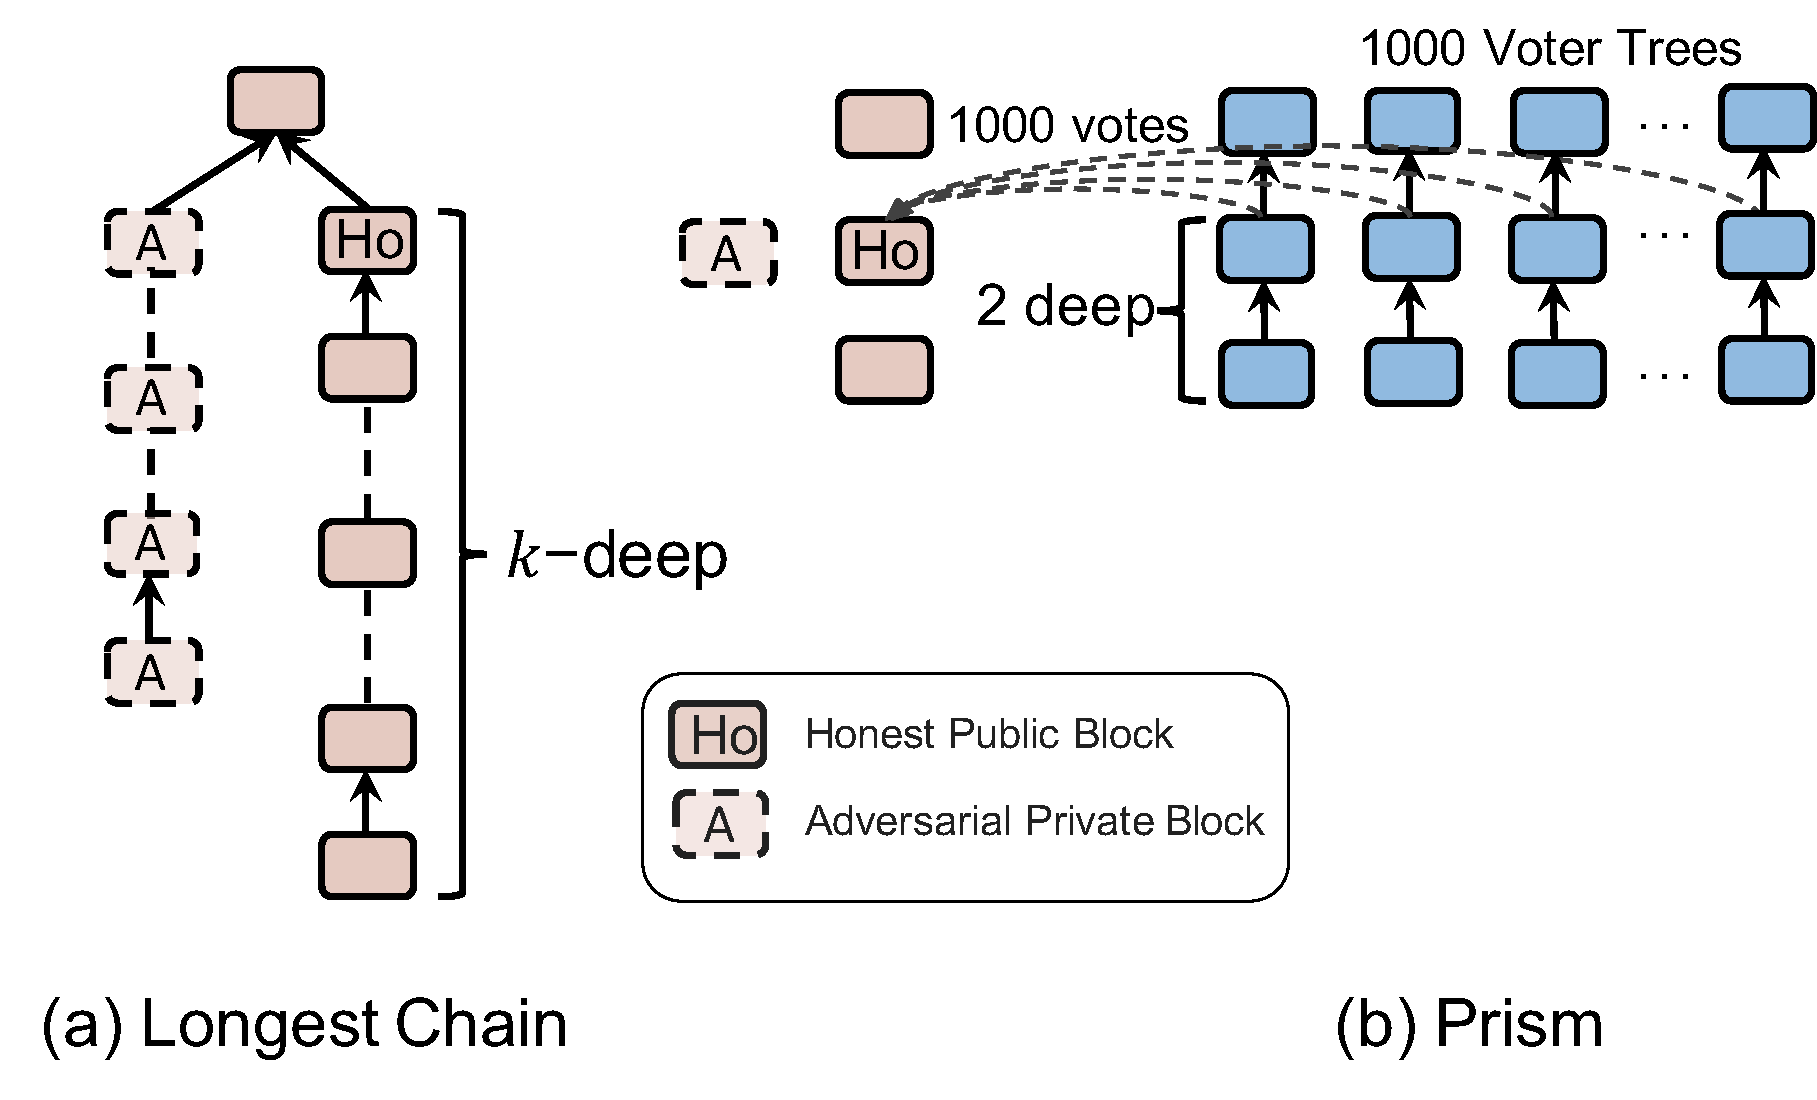
\includegraphics[width=0.75\textwidth]{fast_confirmation_comparision_2.pdf}
\end{center}
\caption{\small Depth of confirmation: longest chain vs. \prism. (a) The longest chain protocol requires a block $Ho$ to be many blocks deep for reliable confirmation, so that an adversary mining in private cannot create a longer chain to reverse block $Ho$. (b) \prism allows each voter block to be very shallow but relies on many voter chains to increase the reliability.}
\label{fig:double_spend}
\end{figure}

\section{Latency Limitation}
\label{s:lc-latency}
A critical attack on the longest chain protocol is the {\em private  double-spend} attack \cite{bitcoin}, as shown in Figure \ref{fig:double_spend}(a). Here, an adversary is trying to revert a block after it is confirmed, by mining a chain in private and broadcasting it when it is longer than the public chain. If the hashing power of the adversary is greater than that of aggregate of the honest nodes, this attack can be easily executed no matter what $k$ is, since the adversary can mine blocks faster on the average than the honest nodes and will eventually  overtake the public chain. On the other hand, when the adversary has less than half the power, the probability of success of this attack can be made exponentially small by choosing the confirmation depth $k$ to be large \cite{bitcoin}. The price to pay for choosing $k$ large is increased latency in confirmation. For example, to achieve a reversal probability of  $0.001$, a depth of $24$ blocks is needed if the adversary has $\beta = 30\%$ of the total hashing power~\cite{bitcoin}.  Figure ~\ref{fig:rd} shows the tradeoff between confirmation depth (and therefore latency) and reliability.


%%With Bitcoin's block mining rate of 1 block every 10 minutes, this translates into a latency of 4 hours! Increasing the block mining rate to, say, 1 block per 10 seconds, improves latency to 240 seconds, but the latency to achieve a high level of reliability is still very high. To achieve a reversal probability of $10^{-6}$, a depth of $50$ blocks is required, translating into a latency of $500$ seconds. Figure ~\ref{fig:rd} shows the tradeoff between confirmation depth (and therefore latency) and reliability. \pv{This is a pretty long section and if we are in a space crunch, then its fine to cut a bit.} 

%In Bitcoin, the mining rate is set much more conservatively, a block roughly every 10 minutes, leading to very long confirmation latency. 

%\ma{I've been assuming this figure also shows the reliability-depth tradeoff for Prism?}
% \begin{figure}
%     \centering
%     \begin{subfigure}[b]{\textwidth}
%         \centering
%         \includegraphics[width=0.35\linewidth]{fast_confirmation_comparision_a.pdf}%
%         \hfill
%         \includegraphics[width=0.35\linewidth]{fast_confirmation_comparision_b.pdf}
%     \end{subfigure}
%     \tion{\small Depth of confirmation: longest chain vs. \prism. (a) The longest chain protocol requires a block to be many blocks deep for reliable confirmation, so that an adversary mining in private cannot create a longer chain. (b) \prism allows each voter block to be very shallow but relies on many voter chains to increase the reliability. \ma{please increase the font size of the subfigure labels, or better, separate this into two figures and use latex's subfig environment}} 
% \end{figure}

\begin{figure}
\begin{center}
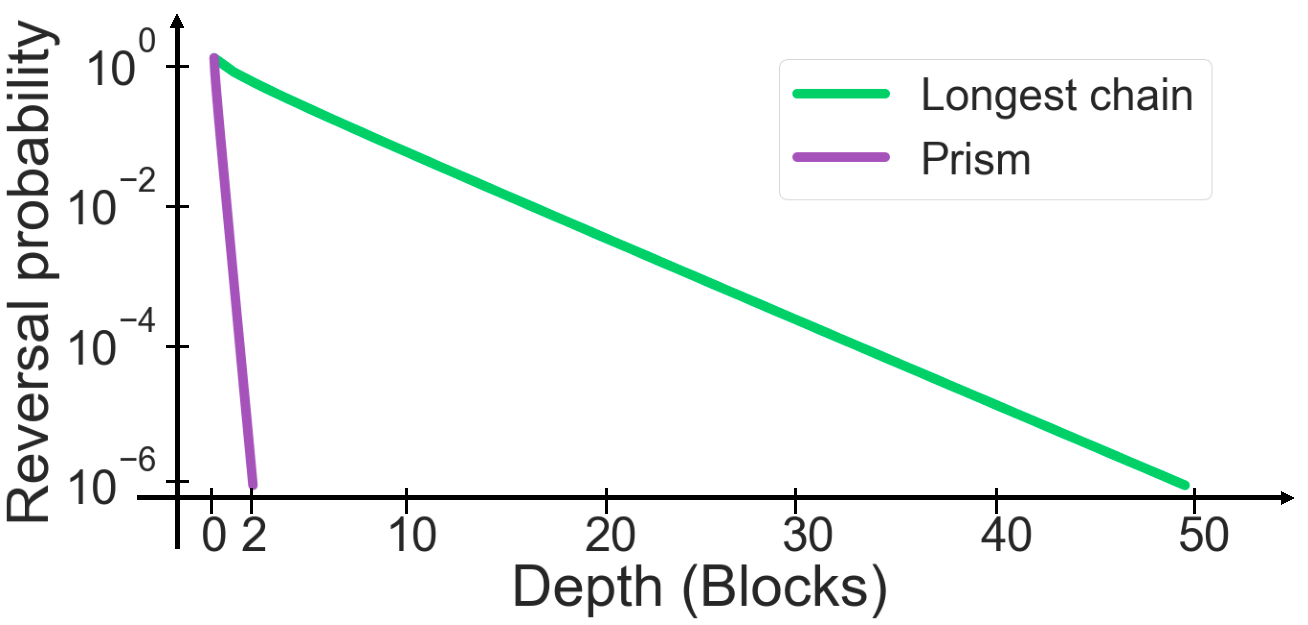
\includegraphics[width=0.6\textwidth]{figures/reliability-depth.pdf}
\end{center}
\caption{\label{fig:rd} \small Reliability as a function of confirmation depth. The reversal probability of \prism has a factor $m$ improvement over the longest chain protocol in the exponential rate of decrease, where $m$ is the number of voter chains (introduced in \S\ref{sec:overview}).}
\end{figure}
\section{Throughput Limitation}
\label{s:lc-thput}

If $B$ is the block size in number of transactions, then the throughput of the longest chain protocol is at most $fB$ transactions per second (tps). 
However, the mining rate $f$ and the block size $B$ are constrained by the security requirement. Increasing the mining rate increases the amount of {\em forking} of the blockchain due to multiple blocks being mined on the same leaf block by multiple miners within the network delay~$\Delta$. Forking reduces throughput since it reduces the growth rate of the longest chain; recall that only blocks on the longest chain contribute to the ledger. More importantly, forking hurts the security of the protocol because the adversary requires less compute power to overtake the longest chain. In fact, the adversarial power that can be tolerated by the longest chain protocol goes from $50\%$ to $0\%$ as the mining rate $f$ increases \cite{backbone}. 
%(Figure \ref{fig:forking}). 
Similarly, increasing the block size $B$ also increases the amount of forking since the network delay $\Delta$ increases with the block size \cite{decker}.

A back-of-the-envelope calculation of the impact of the forking can be done based on a simple model of the network delay: 
$$ \Delta = \frac{hB}{C} + D,$$
where $h$ is the average number of hops for a block to travel, $C$ is the communication bandwidth per link in transactions per second, and $D$ is the end-to-end propagation delay.  This model is consistent with the linear relation between the network delay and the block size as measured empirically by \cite{decker}. 
%\ma{do we have to mention the possibility of cut-through routing? i think we can skip it and maybe mention it in the discussion section towards the end.}
%\vb{Thats a good idea. There are works (like bloxroute) out there which propose cut-through routing to improve the latency.}
Hence, the utilization, i.e. the throughput as a fraction of the communication bandwidth, is upper bounded by
$$ \frac{fB}{C} < \frac{f\Delta}{h},$$
where $f\Delta$ is the average number of blocks ``in flight'' at any given time, and reflects the amount of forking in the block tree.  %%which is nothing but the \textit{forking rate} on the longest chain. \ma{how is forking rate defined?}
In the longest chain protocol, to be secure against an adversary with $\beta < 50\%$ of hash power, this parameter should satisfy \cite{backbone}
$$f\Delta<\frac{1-2\beta}{\beta}.$$
For example, to achieve security against an adversary with $\beta = 45\%$ of the total hashing power, one needs $f\Delta \approx 0.2$. With $h = 5$, this translates to a utilization of at most $4\%$. The above bound holds regardless of block size; the utilization of the longest chain protocol cannot exceed 4\% for $\beta = 45\%$ and $h=5$.
In summary, to not compromise on security, $f\Delta$ must be kept much smaller than $1$. 
Hence, the security requirement (as well as the number of hops) limits the bandwidth utilization.  

%%$$ \ma{I still don't understand why this is different from the analysis in Appendix %%D.2 of the Prism paper.}
%%\vb{The analysis in D.2 is a conservative necessary condition. Whereas the above %%formula is only a necessary condition. It comes from the simple fact that the %%honest nodes grow at rate $\frac{(1-\beta)}{1+f\Delta}$ and adversary grows at rate %%$f\beta$.}
%%\gf{The phrasing above the equation makes it sound like a necessary condition.} %%\vb{Typo. It is indeed a necessary condition

% \ma{Can we state how security depends on $f\Delta$ here precisely, and replace Figure 3 with one that shows maximum possible $f\Delta$ vs. $\beta$. The next sentence gives the specific point $\beta=0.45$ as an example. The nice thing about this is that it highlights that in the longest chain protocol, to meet the security requirement, one cannot have too many blocks in flight at the same time. Prism doesn't have this limitation. However, if my understanding is correct, it will show that $f\Delta$ can be 1 for $\beta < 0.33$, and drops sharply only for higher security levels. This would mean that the possible utilization for Bitcoin in practice is really $1/h$. Is this correct? Prism can only improve throughput from $1/h$ to $1$, unless we're concerned with very high security?} 
% \vb{The effective throughput due to forking is $fB\big(\frac{1}{1+f\Delta}\big)$} \ly{$f\Delta = \frac{1-2\beta}{\beta}$ See Figure~\ref{fig:forking-new}} \ma{Is this consistent with the Prism theory paper, Appendix D.2? I'm still not happy with our explanation here. My hope is that we can remove Fig. 3, and use the fact that f$\Delta$ must be small for security, and the equation above to show that the utilization of the longest chain protocol is limited. @Vivek: please see if this makes sense and update this section.}


%%In summary, in the longest chain protocol, security of the system is fundamentally at odds with low latency and high throughput. To achieve a low reversal probability, blocks must be deep in the longest chain, increasing confirmation latency. At the same time, increasing the mining rate or block size would compromise security because of forking. As we discuss next, \prism removes these limitations to achieve high throughput, low latency, and security simultaneously. 

%\red{GF: Maybe explain in words why we can hope to fix this problem? The dependency on  graph diameter is fundamental, since all honest nodes have to come to consensus, but the effect of Bitcoin's security requirement could  be circumvented by designing a system that trades latency for communication in its confirmation rule.}

\if 0
\begin{figure}
\begin{center}
\includegraphics[width=0.4\textwidth]{figures/forking_security.pdf}
\end{center}
\caption{ Increasing mining rate or block size increases forking and reduces security. 
\red{GF: Are we going to add numbers to the x-axis? This looks a bit cartoonish, I think having actual nubmers on the axes would help,  if we want to keep this figure at all (not sure it clarifies too much?).} \ly{Shall I redo the plot to put numbers on x-axis and make it the same style as figure 8 to 12?}
\vb{I have added numbers to x-axis for now.}
\gw{Caption says "or block size", but it's not in the figure.}}
\label{fig:forking}
\end{figure}

\fi

% \begin{figure}
% \centering
% \input{figures/fdelta-fig.tex}
% \caption{ Increasing mining rate or block size increases forking and reduces security. \gw{Is this the correct caption for the figure?}} \ma{No. This figure might actually work better with $f\Delta$ on the x-axis. The focus should probably be the region where $f\Delta$ is small, say less than 2 or 3. I'm not sure the figure is correct. @Vivek: please double check} \vb{This figure look correct}
% \label{fig:forking-new}
% \end{figure}




